\chapter{Tool description}
\label{cap:toolDescription}
DDC consists of approximately 900 lines of mostly statically typed Python, which can be found in \url{https://github.com/RCoeurjoly/DDC/blob/main/declarative_debugger.py}.
%
It is loaded into rr through the source command, which itself can be put inside a \verb|.gdbinit| file.
%
In this chapter we will explain the architecture of the tool.
Then, we will go through two usage scenarios:
\begin{itemize}
    \item Bug finding.
    \item Using test cases as oracles to reduce tree size.
\end{itemize}
Lastly, we will list all commands provided by the tool.

\section{Architecture}
In this section we detail and justify the most important design decisions made while developing DDC.
\subsection{Tree building}
To represent the debugging tree, we use the \verb|Node| class. The \verb|Node| class is a recursive data structure, since it has an attribute called \verb|children| which is a list of \verb|Node|s. This list of children nodes are sorted by execution time, that is, children node in position \(n\) has executed before than children node in position \(n+1\).

The \verb|DebuggingSession| class has attribute of type \verb|Node| to store the debugging tree. It also tracks if the debugging session has begun and if the tree has been built.

\subsubsection{Adding a node to the tree}
We add a node to the debugging tree once we hit a breakpoint.
The node is added to the last position of the tree.
At that moment we add the 3-tuple of inputs to the node.
\subsubsection{Finishing a node}
When the finish breakpoint of a certain function it hit, we add the 4-tuple of outputs.
\subsubsection{Finishing the tree building process}
The tree is considered built if one of the following happens:
\begin{itemize}
    \item A final point has been hit.
    \item The program has finished.
    \item The root node has been completed.
\end{itemize}
\subsection{Tree transformations}
After having the WMDT built, we apply all tree transformations available.
A tree transformation is an algorithm that receives a WMDT an returns another WMDT.
DDC implements for the simplified tree compression algorithm, which is described next.
\subsubsection{Simplified tree compression}
The simplified tree compression algorithm consists in two steps:
\begin{itemize}
    \item Compressing the root of the WMDT if it can be compressed.
    \item Compressing each of the children nodes of the root of the WMDT if they can be compressed.
\end{itemize}
Given a WMDT, we can compress nodes if:
\begin{itemize}
    \item The root node has only one child node.
    \item The root and child nodes function names are the same.
\end{itemize}
To check if a node can be compressed we use a recursive function, which takes a node as an argument and returns a 2-tuple, whose elements are:
\begin{itemize}
    \item bool: True if the node can be compressed. False otherwise.
    \item int: If the node can be compressed, number of nodes to compress. Zero Otherwise.
\end{itemize}
This algorithm searches for the longest compression possible.

Given a WMDT and a number of nodes to compress \(n\), the compress node is composed of:
\begin{itemize}
    \item The 3-tuple of inputs to the root node.
    \item The 4-tuple of outputs of the node in depth \(n\) of the WMDT.
    \item The name of the root node with an indication that corresponds to \(n\) compressed nodes.
\end{itemize}

\subsection{General debugging algorithm}
The general debugging algorithm takes two arguments:
\begin{itemize}
    \item The WMDT.
    \item A navigation strategy.
\end{itemize}
It returns either a buggy node or \(\bot\).
It consists of loop, from which we exit if the WMDT is empty or a buggy node has been found.
To determine if a node has been found we have to check that the WMDT consists of an unique incorrect node.

Once inside the loop, first we select the node to be asked about by means of the strategies, which are explained in \hyperref[implementation:Strategies]{Section Strategies}.
We then ask the user about the node. One of the options available to the user is to change strategy. If this is chosen, we ask the user her preferred strategy and continue the execution of the loop.

If no change in strategy is required, we execute the adequate action corresponding to the correctness answer (see \hyperref[implementation:correctnessAnswers]{Section User answers to correctness questions}) and continue the execution of the loop.

\subsection{Navigation strategies}
\label{implementation:Strategies}
A navigation strategy is an algorithm that takes a WMDT and returns a node.
In the implementation we also need to keep track of the position of the current node, since Top-down is a recursive algorithm.

To ease the task of adding more strategies to DDC, we implemented a wrapper to the strategies.

\subsubsection{Top-down}
Top-down is a recursive algorithm, which searches for the first node whose correctness is unknown.

\subsubsection{Divide and Query (Hirunkitti)}
In Divide and Query (Hirunkitti), we select the child node whose weight is the closest to half of the root node weight.

\subsubsection{Heaviest first}
In heaviest first, we select the child node whose weight is the heaviest.

\subsection{User answers to correctness questions}
\label{implementation:correctnessAnswers}
When asked about the correctness of a node, the user has the possibility of answering (i) I don't know, (ii) Yes, (iii) No or (iv) Trusted.
We choose the next node and/or prune the debugging tree depending on the answer
\subsubsection{I don't know}
If the user does not know if the node is correct, we remove it from the WMDT and continue the debugging session.
\subsubsection{Yes}
If the node is deemed correct by the user, we remove it from the WMDT and all other nodes equal to the correct node.

\subsubsection{No}
If the node is deemed incorrect by the user, we continue the navigation phase with this node as the WMDT root.
\subsubsection{Trusted}
If the node is trusted by the user, we remove it from the WMDT and all other nodes which correspond to executions of the same function of the correct node.


\subsection{Test cases as oracles}
DDC implements the functionality of test cases as oracles with two global variables:

\begin{itemize}
    \item In \verb|CORRECT_NODES| we store a list of all nodes that have finished, that is, whose functions have returned.
    \item In \verb|PENDING_CORRECT_NODES| we store a list of all nodes that have started but not finished.
\end{itemize}

To compare the gathered correct nodes with those within the debugging tree, we implement the \verb|ComparableTree| class that derives from \verb|rich.tree|, which is the class used to present the information to the user.

The \verb|Node| class has a member function \verb|get_tree|, which returns a \verb|ComparableTree|.
For comparison with elements in the \verb|CORRECT_NODES| list, the node gets stripped of its correctness value, children and weight.

Once a node finishes, we search for it in the \verb|CORRECT_NODES| list. If found, we remove it from the debugging tree.

\section{Usage scenarios}
This section describes two usage scenarios with DDC.
We will explain which commands should be executed and the expected output.

\subsection{Bug finding}
The execution of the code in Figure~\ref{lst:unexpectedQuicksortSource} results in an unexpected output, \(\{10, 5, 1, 7, 8, 9\}\), which is not sorted.
It uses the implementations of functions \verb|quickSort|, \verb|partition|, and \verb|swap| defined in Figure~\ref{lst:quicksortFunctions}.
\begin{lstlisting}[language=C++, caption={Code that results in unexpected output}, frame=tb, label={lst:unexpectedQuicksortSource}]
#include <quicksort.h>

int main()
{
  std::vector<int> my_vector{ 10, 7, 8, 9, 1, 5 };
  quickSort(my_vector, 0, my_vector.size()-1);
  std::cout << "Sorted vector: " << std::endl;
  print_vector(my_vector);
  return 0;
}
\end{lstlisting}

\begin{lstlisting}[language=C++, caption={quickSort, partition and swap implementations}, frame=p, label={lst:quicksortFunctions}]
#include <iostream>
#include <vector>

void swap(int* a, int* b)
{
  if (*a != 10)
    std::swap(*a, *b);
}

int partition(std::vector<int> &my_vector, int low, int high)
{
  int pivot = my_vector[high];
  int i = (low - 1);
  for (int j = low; j <= high - 1; j++)
    {
      if (my_vector[j] <= pivot)
        {
          i++;
          if (i != j)
            swap(&my_vector[i], &my_vector[j]);
        }
    }
  if ((i + 1) != high)
    swap(&my_vector[i + 1], &my_vector[high]);
  return (i + 1);
}

void quickSort(std::vector<int> &my_vector, int low, int high)
{
  if (low < high)
    {
      int pi = partition(my_vector, low, high);
      quickSort(my_vector, low, pi - 1);
      quickSort(my_vector, pi + 1, high);
    }
}

void print_vector(const std::vector<int> &my_vector)
{
  for (size_t i = 0; i < my_vector.size(); i++) {
    std::cout << my_vector[i] << ' ';
  }
}
\end{lstlisting}

To begin a debugging session with the purpose of finding the cause of the error, we first have to record and replay the buggy program with \verb|rr|. This is shown in
Figure~\ref{lst:compileRecordReplayQuicksort}.
\begin{lstlisting}[language=bash, caption={Compiling, recording and replaying quickSort}, frame=tb, label={lst:compileRecordReplayQuicksort}]
nix build
rr record ./result/bin/quicksort
rr replay
\end{lstlisting}
Once inside the \verb|rr| command prompt, we have to tell DDC in which functions we suspect the bug to reside.
To do this, we use the \verb|suspect-function| command described in command \hyperref[command:suspect-function]{suspect-function}\todo{A menudo pones ref pero no Figure o lo que sea, revisar. Además, Figure va con mayúscula (ha cambiado varias, pero revisar)}. In this case, we suspect the functions we defined, that is, \verb|quickSort|, \verb|partition|, and \verb|swap|. We execute the commands shown in Figure \ref{fig:suspecting-functions} in \verb|rr|.
\begin{figure}[h]
    \centering
    \caption{Setting the suspect functions}
    \label{fig:suspecting-functions}
    \begin{verbatim}
(rr) suspect-function quickSort(std::vector<int>&, int, int)
Breakpoint 1 at 0x40135e: file quicksort.h, line 44.
(rr) suspect-function partition(std::vector<int>&, int, int)
Breakpoint 2 at 0x401256: file quicksort.h, line 20.
(rr) suspect-function swap(int*, int*)
Breakpoint 3 at 0x401222: file quicksort.h, line 9.
(rr) info breakpoints
Num Type       Disp Enb Address         What
1   breakpoint keep y   0x40135e in quickSort(std::vector<int>&, int, int)
    add-node-to-session quickSort(std::vector<int>&, int, int)
2   breakpoint keep y   0x401256 in partition(std::vector<int>&, int, int)
    add-node-to-session partition(std::vector<int>&, int, int)
3   breakpoint keep y   0x401222 in swap(int*, int*)
    add-node-to-session swap(int*, int*)
    \end{verbatim}
\end{figure}
Note that the results of the command \verb|info breakpoints| have been simplified for display purposes.
Now we can choose the navigation strategy.
\begin{figure}[h]
    \centering
    \caption{Choosing the navigation strategy}
    \label{fig:navigationsStrategyPrompt}
    \begin{verbatim}
Please choose navigation strategy
> Top-down
  Divide and Query (Hirunkitti)
  Heaviest first
    \end{verbatim}
\end{figure}
Then, as shown in Figure \ref{fig:correctnessQuestion}, the debugger asks us about the correctness of the root node of the debugging tree. This question does not have the option to change the navigation strategy, as opposed to all other correctness questions, where the options are shown in Figure \ref{fig:correctnessQuestionNonRootOptions}.

\begin{figure}[h]
    \centering
    \caption{Correctness question of root node}
    \label{fig:correctnessQuestion}
    \begin{verbatim}
You have selected Top-down!
Is the following node correct?
quickSort(std::vector<int, std::allocator<int> >&, int, int)
├── correctness
│   └── I don't know
├── weight
│   └── 14
├── arguments on entry
│   ├── my_vector = std::vector of length 6, capacity 6 = {
│   │     [0] = 10,
│   │     [1] = 7,
│   │     [2] = 8,
│   │     [3] = 9,
│   │     [4] = 1,
│   │     [5] = 5
│   │   }
│   ├── low = 0
│   └── high = 5
└── arguments when returning
    └── my_vector = std::vector of length 6, capacity 6 = {
          [0] = 10,
          [1] = 5,
          [2] = 1,
          [3] = 7,
          [4] = 8,
          [5] = 9
        }
> Yes
  No
  I don't know
  Trusted
    \end{verbatim}
\end{figure}

\begin{figure}[h]
    \centering
    \caption{Options to correctness question of non root node}
    \label{fig:correctnessQuestionNonRootOptions}
    \begin{verbatim}
> Yes
  No
  I don't know
  Trusted
  Change strategy
    \end{verbatim}
\end{figure}

The debugging session ends when the buggy node is found, as shown in Figure \ref{fig:buggyNodeFound}. Although we only have the granularity to say which function is buggy, we also display with what inputs the buggy function misbehaves, so that the user can create a test case that reproduces the failure.
\begin{figure}[h]
    \centering
    \caption{Buggy node found}
    \label{fig:buggyNodeFound}
    \begin{verbatim}
Buggy node found
swap(int*, int*)
├── arguments on entry
│   ├── a = 10
│   └── b = 1
└── arguments when returning
    ├── a = 10
    └── b = 1
    \end{verbatim}
\end{figure}

\subsection{Using test cases as oracles to reduce tree size}
Now, using the same buggy program as in the previous section, we are going to gather correct nodes by executing test cases.
To do this, we first have to develop a C++ executable which uses the functions with suspect to be buggy, which we display in Figure \ref{lst:quicksortTests}.
\begin{lstlisting}[language=C++, caption=Test cases for quickSort, frame=tb, label={lst:quicksortTests}]
#include <quicksort.h>
#include <algorithm>
#include <cassert>

int main()
{
  std::vector<int> my_vector{ 0, 0, 0, 0, 0, 0 };
  const int n = 6;
  for (int i = 0; i <= 9; i++) {
    my_vector[0] = rand() % 9 + 1;
    my_vector[1] = rand() % 9 + 1;
    my_vector[2] = rand() % 9 + 1;
    my_vector[3] = rand() % 9 + 1;
    my_vector[4] = rand() % 9 + 1;
    my_vector[5] = rand() % 9 + 1;
    quickSort(my_vector, 0, n-1, "");
    if (!std::is_sorted(my_vector.begin(), my_vector.end()))
      return 1;
  }
  return 0;
}
\end{lstlisting}
In this listing, we see that we test ten vectors composed of random numbers from 0 to 9. When executing these test cases, the return code is 0, so we know that our \verb|quickSort| implementation at least works for some vectors.

Like with a buggy program, we first have to record the execution with \verb|rr|. This shell will be named \(rr_{server}\), to differentiate it from the debugging shell.
\begin{lstlisting}[language=bash, caption={Compiling, recording and replaying quickSort test cases}, frame=tb, label={lst:compileRecordReplayQuicksortTests}]
nix build .#test_quicksort
rr record ./result/tests/test_quicksort
rr replay
\end{lstlisting}
Once inside the \verb|rr| command prompt, we have to tell DDC from which functions should the correct nodes be gathered.
This can be done with the \verb|save-correct-function| command described in the command \hyperref{command:save-returning-correct-node}[save-returning-correct-node]. In our example, we want to save correct nodes gathered from the functions we defined, that is, \verb|quickSort|, \verb|partition| and \verb|swap|. Therefore, we execute the commands shown in Figure \ref{fig:saving-correct-functions} in \verb|rr|. Again, the results of the command \verb|info breakpoints| have been simplified.
\begin{figure}[h]
    \centering
    \caption{Setting the functions from which to gather correct nodes}
    \label{fig:saving-correct-functions}
    \begin{verbatim}
(rr) save-correct-function quickSort(std::vector<int>&, int, int)
Breakpoint 1 at 0x40135e: file quicksort.h, line 44.
(rr) save-correct-function partition(std::vector<int>&, int, int)
Breakpoint 2 at 0x401256: file quicksort.h, line 20.
(rr) save-correct-function swap(int*, int*)
Breakpoint 3 at 0x401222: file quicksort.h, line 9.
(rr) info breakpoints
Num Type       Disp Enb Address         What
1   breakpoint keep y   0x40135e in quickSort(std::vector<int>&, int, int)
    add-node-to-correct-list quickSort(std::vector<int>&, int, int)
2   breakpoint keep y   0x401256 in partition(std::vector<int>&, int, int)
    add-node-to-correct-list partition(std::vector<int>&, int, int)
3   breakpoint keep y   0x401222 in swap(int*, int*)
    add-node-to-correct-list swap(int*, int*)
    \end{verbatim}
\end{figure}

At this point, we can use the \verb|GDB| commands \verb|start| and \verb|continue| (this last one repeatedly) to reach the end of the program.
Alternatively, we have provided the convenience command \verb|til-the-end| (see command \hyperref{command:til-the-end}[til-the-end]) that has the exact same functionality.
Once we have reached the end of the program, all nodes have been collected. This can be checked by dropping into an interactive Python shell inside \verb|rr| like is shown in Figure \ref{fig:python-interactive}. To exit the Python shell, use \verb|Ctrl-D|.
\begin{figure}[h]
    \centering
    \caption{Starting an interactive Python shell inside rr}
    \label{fig:python-interactive}
    \begin{verbatim}
    (rr) python-interactive
    >>>
    \end{verbatim}
\end{figure}
Once inside the shell, we can examine the set of correct nodes. For example, we can check how many correct nodes we have gathered (see Figure~\ref{fig:lengthLists}) or display any of those nodes (see Figure \ref{fig:printCorrectNode}).
\begin{figure}[h]
    \centering
    \caption{Length lists}
    \label{fig:lengthLists}
    \begin{verbatim}
    >>> len(CORRECT_NODES)
    156
    >>> len(PENDING_CORRECT_NODES)
    0
    \end{verbatim}
\end{figure}

\begin{figure}[h]
    \centering
    \caption{Printing a correct node}
    \label{fig:printCorrectNode}
    \begin{verbatim}
>>> print_tree(CORRECT_NODES[0])
partition(std::vector<int, std::allocator<int> >&, int, int)
├── arguments on entry
│   ├── my_vector = std::vector of length 6, capacity 6 = {
│   │     [0] = 2,
│   │     [1] = 8,
│   │     [2] = 1,
│   │     [3] = 8,
│   │     [4] = 6,
│   │     [5] = 8
│   │   }
│   ├── low = 0
│   └── high = 5
├── arguments when returning
│   └── my_vector = std::vector of length 6, capacity 6 = {
│         [0] = 2,
│         [1] = 8,
│         [2] = 1,
│         [3] = 8,
│         [4] = 6,
│         [5] = 8
│       }
└── return value
    └── 5
    \end{verbatim}
\end{figure}
Once all correct nodes have been collected, we have to start the debugging session of our buggy program with a separate \verb|rr| execution (see Figure \ref{lst:compileRecordReplayQuicksort}), which we will call \(rr_{client}\), and collect the correct nodes already gathered from \(rr_{server}\). This has to be done with the command \verb|listen-for-correct-nodes}| (see command \hyperref{command:listen-for-correct-nodes}[listen-for-correct-nodes]).

Now we are ready to send the correct nodes from \(rr_{server}\) to \(rr_{client}\). This is done with the command \verb|send-correct-nodes| (see command \hyperref{command:send-correct-nodes}[send-correct-nodes]).
In \(rr_{server}\) we can see that nodes are being sent, like shown in Figure \ref{fig:sendingNode}.
\begin{figure}[h]
    \centering
    \caption{Sending nodes to client}
    \label{fig:sendingNode}
    \begin{verbatim}
    Sending node n# 87
    \end{verbatim}
\end{figure}
Likewise, in \(rr_{client}\) we can see that nodes are being received, like shown in Figure \ref{fig:receivingNode}.
\begin{figure}[h]
    \centering
    \caption{Receiving nodes from server}
    \label{fig:receivingNode}
    \begin{verbatim}
    Connected by ('127.0.0.1', 51126)
    \end{verbatim}
\end{figure}

\begin{figure}[p]
\centering
    \caption{Zoomable tree of buggy quickSort after correct node elimination}
    \label{fig:buggyTreeAfter}
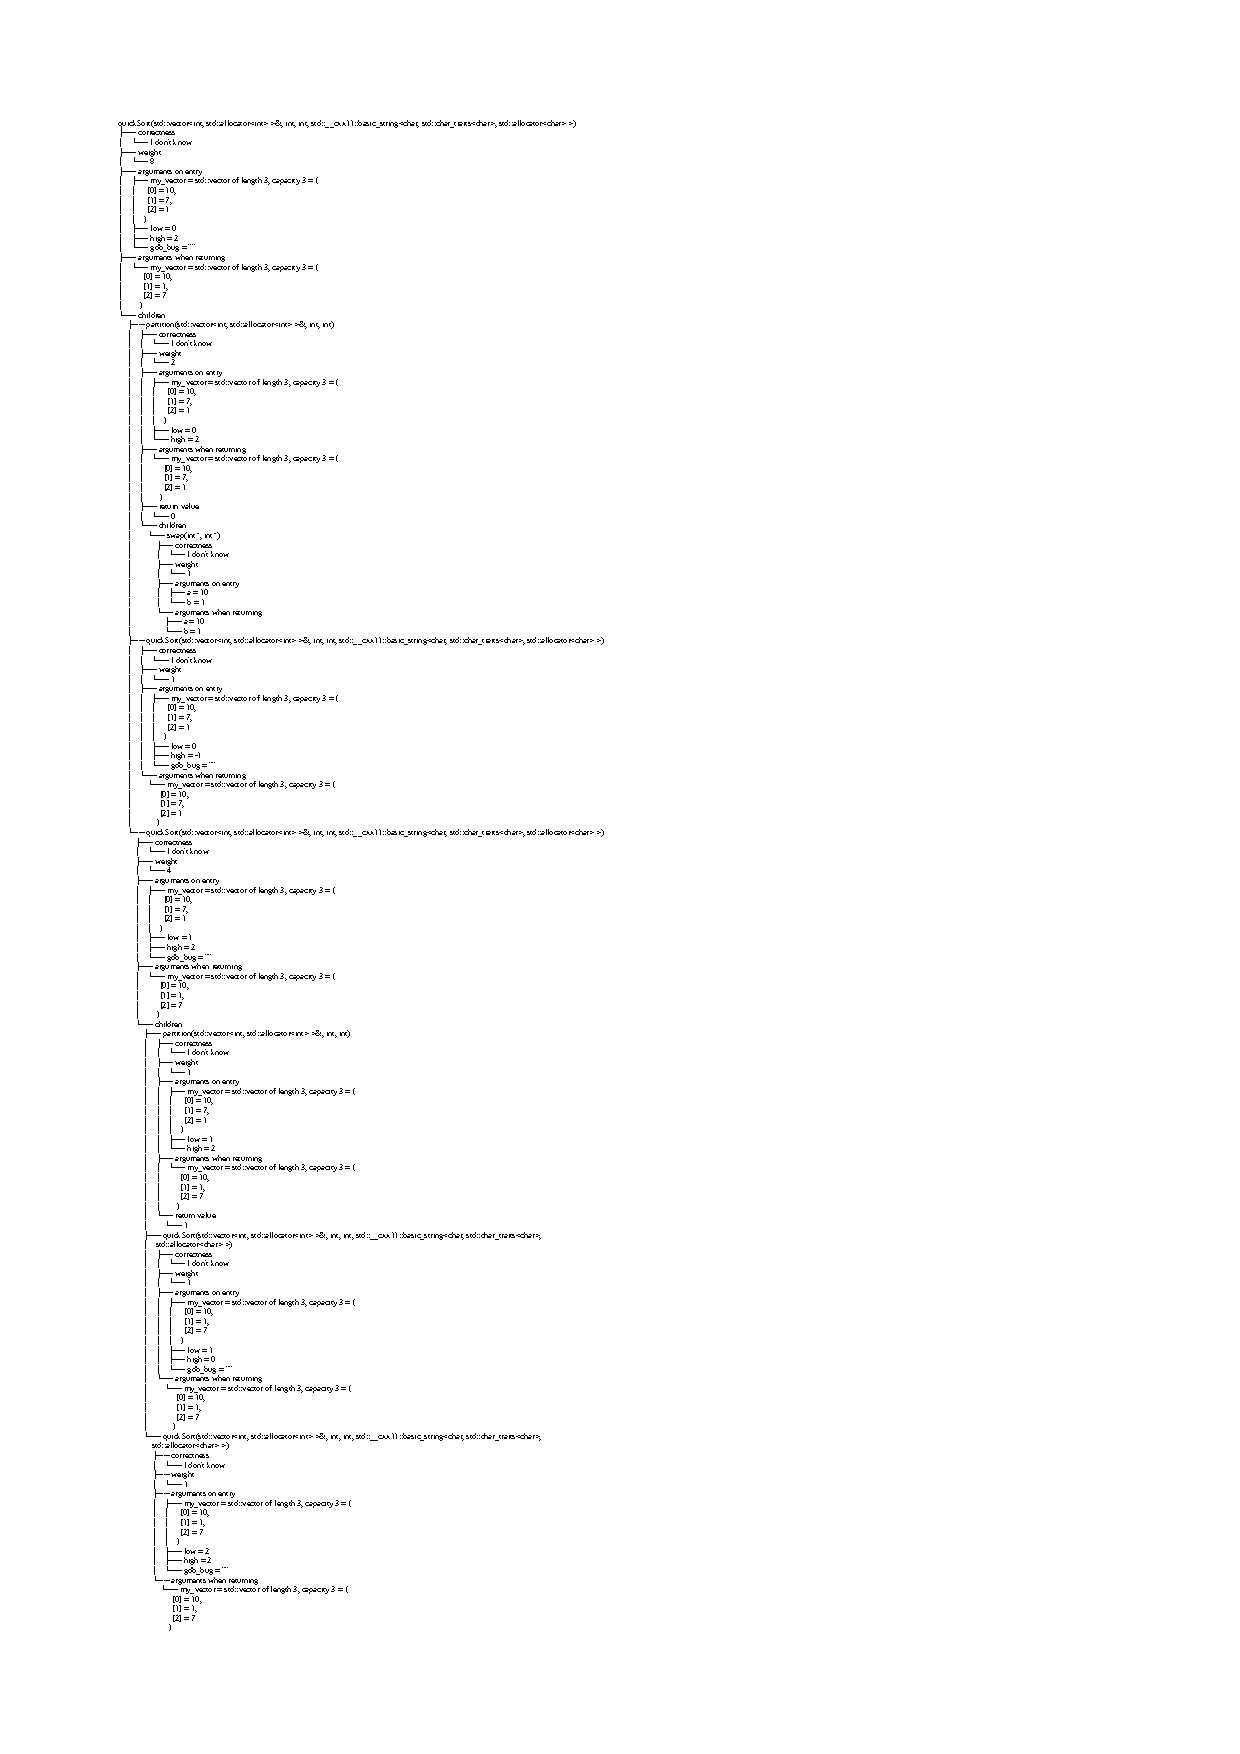
\includegraphics[width=\textwidth,height=\textheight,keepaspectratio]{Imagenes/Vectorial/buggySwapRemoved.pdf}
\end{figure}

%\begin{figure}
%\centering
%\caption{Correct node removed from debugging tree}
%\label{fig:removedNode}
%\begin{verbatim}
%swap(int*, int*)
%├── arguments on entry
%│   ├── a = 7
%│   └── b = 1
%└── arguments when returning
%    ├── a = 1
%    └── b = 7
%\end{verbatim}
%\end{figure}
\begin{figure}[p]
\centering
    \caption{Prueba}
    \label{fig:correctNodeRemoved}
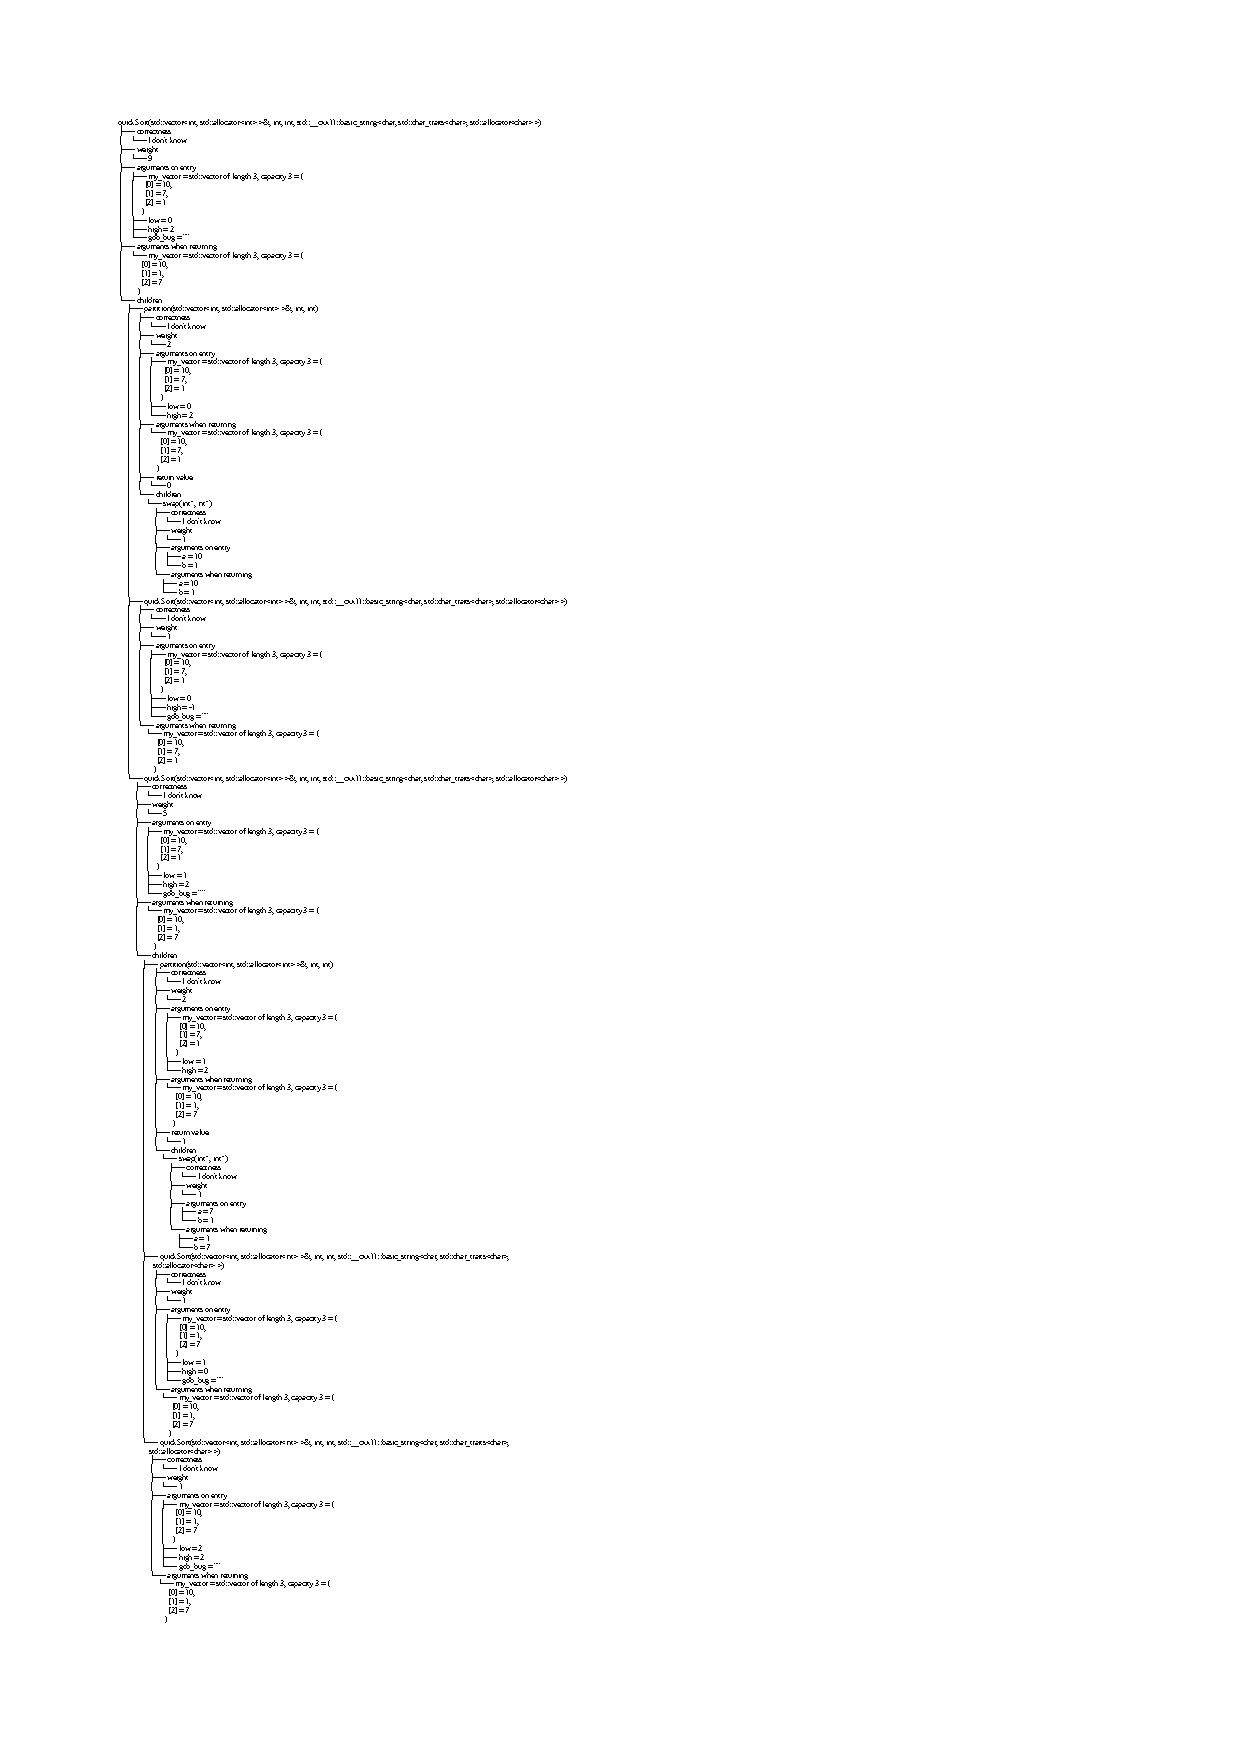
\includegraphics[width=\textwidth,height=\textheight,keepaspectratio]{Imagenes/Vectorial/buggy.pdf}
\end{figure}
If we now start the debugging session (after setting the suspect functions like demonstrated in Figure \ref{fig:suspecting-functions}\todo{Ojo}), we see that the WMDT has 8 nodes (see Figure \ref{fig:buggyTreeAfter}) instead of 9 (see Figure \ref{fig:buggyTreeBefore}). This is because a swap node has been removed, more specifically, the node in Figure \ref{fig:correctNodeRemoved}.


This node has been removed from the debugging tree because it appeared in a test case, therefore the debugger has deduced that this computation is correct.
\section{Benchmarking}

\begin{figure}
    \centering
    \begin{gnuplot}[terminal=pdf]
    set logscale x
    set xlabel "Input vector length (elements)"
    set logscale y
    set ylabel "Time (nanoseconds)"
    set xrange [1:200000]
    set yrange [1000000:200000000000]
    plot 'Datos/executing_quicksort.dat' using 1:2 title "Execution", 'Datos/recording_quicksort.dat' using 1:2 title "Recording", 'Datos/tree_building_quicksort.dat' using 1:2 title "Tree building"
    \end{gnuplot}
    \caption{Quicksort execution vs record vs tree building}
\end{figure}

\begin{figure}
    \centering
    \begin{gnuplot}[terminal=pdf]
    set logscale x
    set xlabel "Number of nodes"
    set logscale y
    set ylabel "Time (nanoseconds)"
    set xrange [1:1000]
    set yrange [100000000:100000000000]
    plot 'Datos/nodes_vs_time.dat' using 1:2
    \end{gnuplot}
    \caption{Nodes vs time}
\end{figure}
%2 2258950
%131072 259707785
2 360308717 
4 718401324 
8 1408922217 
16 2730037241 
32 6156850321 
64 13337290712 
128 32220226111 
256 87456416294 

\section{Commands}
We now list and describe all the available commands. These can be issued inside rr. Completion for these commands is enabled, that is, if you type \verb|sus| and then \verb|TAB|, \verb|suspect-function| should appear.
The following information can also be found with \verb|help <command>|, where \verb|<command>| is one of the commands that follow.

\begin{enumerate}
    \item suspect-function
\label{command:suspect-function}

Mandatory command used in a debugging session.

Sets a breakpoint on the location provided as argument. It also adds the command \hyperref[command:add-node-to-session]{add-node-to-session} to it.
It should be used at least once before starting the debugging session.

Arguments: location.

Location completion is enabled.


\item add-node-to-session
\label{command:add-node-to-session}

Optional command used in a debugging session.
Adds the current frame to the debugging tree.
It expects to be called on entry to a function or method.
It also creates a finish breakpoint for the current function or method, with the attach command \hyperref[command:save-returning-node]{save-returning-node}.

It can be used to create an ad hoc debugging tree.

It is used by \hyperref[command:suspect-function]{suspect-function}.

Arguments: none.
\item save-returning-node
\label{command:save-returning-node}

It saves the arguments of the function or method that just returned.
This is the command attached to finish breakpoints created with \hyperref[command:add-node-to-session]{add-node-to-session}.

For internal use only.

Arguments: none.
\item final-point
\label{command:final-point}

Optional command used in a debugging session.
Sets a breakpoint on the location provided as argument and adds the command \hyperref[command:finish-debugging-session]{finish-debugging-session} to it.
It can be used zero or more times.

Arguments: location.

Location completion is enabled.
\item finish-debugging-session
\label{command:finish-debugging-session}

Sets the Boolean variable describing that the tree has been built to true.
This command is executed when a \hyperref[command:final-point]{final-point} is reached.

Internal use only.

Arguments: none.
\item start-declarative-debugging-session
\label{command:start-declarative-debugging-session}

Mandatory command used in a debugging session.
If the debugging tree has not been built, it builds it. Otherwise, it starts to ask correctness questions to the user.

Arguments: none.
\item save-correct-function
\label{command:save-correct-function}

Sets a breakpoint on the location provided as argument, setting as command \hyperref[command:save-returning-correct-node]{save-returning-correct-node}. Mandatory command used in gathering correct nodes.

Arguments: location.

Location completion is enabled.
\item add-node-to-correct-list
\label{command:add-node-to-correct-list}

Optional command used in gathering correct nodes.
Adds the current frame to the debugging tree.
It expects to be called on entry to a function or method.
It also sets a final breakpoint on current function or method, with the attached command \hyperref[command:save-returning-correct-node]{save-returning-correct-node}.

Arguments: none.

For internal use only.
\item save-returning-correct-node
\label{command:save-returning-correct-node}

It saves the arguments of the function or method that just returned into the appropriate node.

Arguments: none.

For internal use only.
\item til-the-end
\label{command:til-the-end}

Continues the execution of the inferior until the program is not being run.

Optional command used in gathering correct nodes.

Arguments: none.
\item listen-for-correct-nodes
\label{command:listen-for-correct-nodes}

Open a connection on localhost, port 4096, and wait for correct nodes to be sent.

Executed by the client.
Mandatory command used in gathering correct nodes.
Must be executed before calling \hyperref[command:send-correct-nodes]{send-correct-nodes} in the server.

Arguments: none.
\item send-correct-nodes
\label{command:send-correct-nodes}

Send all the correct nodes gathered from tests to the client.
Executed by the server.
The client has to have issued the \hyperref[command:listen-for-correct-nodes]{listen-for-correct-nodes} before, otherwise a ConnectionRefusedError exception is thrown.

Mandatory command used in gathering correct nodes.

Arguments: none.
\item print-tree
\label{command:print-tree}

Prints the debugging tree.
An exception is thrown if the debugging tree has not been built yet.
Optional command that can be used in a debugging session.

Arguments: none.
\end{enumerate}
